\documentclass[12pt]{article}

\usepackage{graphicx}
\usepackage{booktabs}
\usepackage{array}
\usepackage{url}
\usepackage{amsmath}
\usepackage{geometry}
\geometry{margin=1in}

\begin{document}

\title{Pilot-Scale Text Column Detection and Reading-Order Recovery for Traditional Mongolian Historical Archives}

\author{\parbox{0.95\textwidth}{\centering Lanying Liang$^{1}$ \quad Yuefeng Liu$^{2,*}$\\[0.4em]\small $^{1}$Archives, Inner Mongolia University of Science and Technology,\\\small Baotou, 014010, Inner Mongolia, China\\\small $^{2}$School of Digital and Intelligent Industry (School of Cyber Science and Technology),\\\small Inner Mongolia University of Science and Technology, Baotou, 014010, Inner Mongolia, China\\\small *Corresponding author: liuyuefeng@imust.edu.cn; Lanying Liang: 389647973@qq.com}}
\date{}
\maketitle

\begin{abstract}
Traditional Mongolian historical archives pose a challenging page-level document analysis problem because the script is vertically written, cursive, low-resource, and frequently degraded by aging paper, ink variation, seals, scanning rotation, and heterogeneous archive sources. Since expert transcription of handwritten traditional Mongolian columns is expensive and currently unavailable, this concise study focuses on an upstream stage for archival OCR: text-column detection and reading-order recovery. We construct a page-level annotation protocol with text-column bounding boxes, ignored noise regions, orientation metadata, and reading order. We compare classical rule-based extraction, YOLOv8n, and a COCO-pretrained Faster R-CNN MobileNet detector with a rotation-aware ordering strategy. On an independent 11-page test split, YOLOv8n improves the project-level IoU@0.5 F1 score from 0.582 to 0.820 and achieves 0.900 reading-order accuracy, while Faster R-CNN reaches 0.823 F1 after fine-tuning. We provide a crop-export-ready interface, but do not report CER/WER because expert column-level transcripts are not yet available. The study contributes an initial pilot-scale, partially reproducible layout-analysis benchmark for subsequent traditional Mongolian archival OCR research, subject to archive-image access restrictions.
\end{abstract}

\noindent\textbf{Keywords:} Historical document analysis; Traditional Mongolian archives; Text column detection; Reading order recovery; Low-resource document analysis

\section{Introduction}
Full-page recognition of traditional Mongolian historical archives requires more than a recognizer trained on isolated text lines. Pages often contain many vertical handwritten columns, irregular spacing, red seals, page borders, paper stains, and inconsistent scan orientations. If columns are not localized and ordered reliably, downstream OCR modules receive incomplete or misordered crops.

In the current project stage, expert transcription of handwritten traditional Mongolian archive columns is not available. Rather than reporting unverifiable OCR accuracy, this paper evaluates the upstream page-layout problem using bounding-box and reading-order annotations. Layout annotation is cheaper than full transcription and provides the bridge between scanned archive pages and later recognition modules.

Our contributions are threefold. First, we define a page-level annotation protocol for traditional Mongolian archives, including text-column boxes, ignore regions, orientation, and reading order. Second, we provide a pilot-scale benchmark of rule-based and learning-based column detection under a unified matching protocol. Third, we implement a crop-export-ready interface while clearly separating layout evaluation from future transcription-based OCR evaluation.

\begin{figure}[t]
\centering
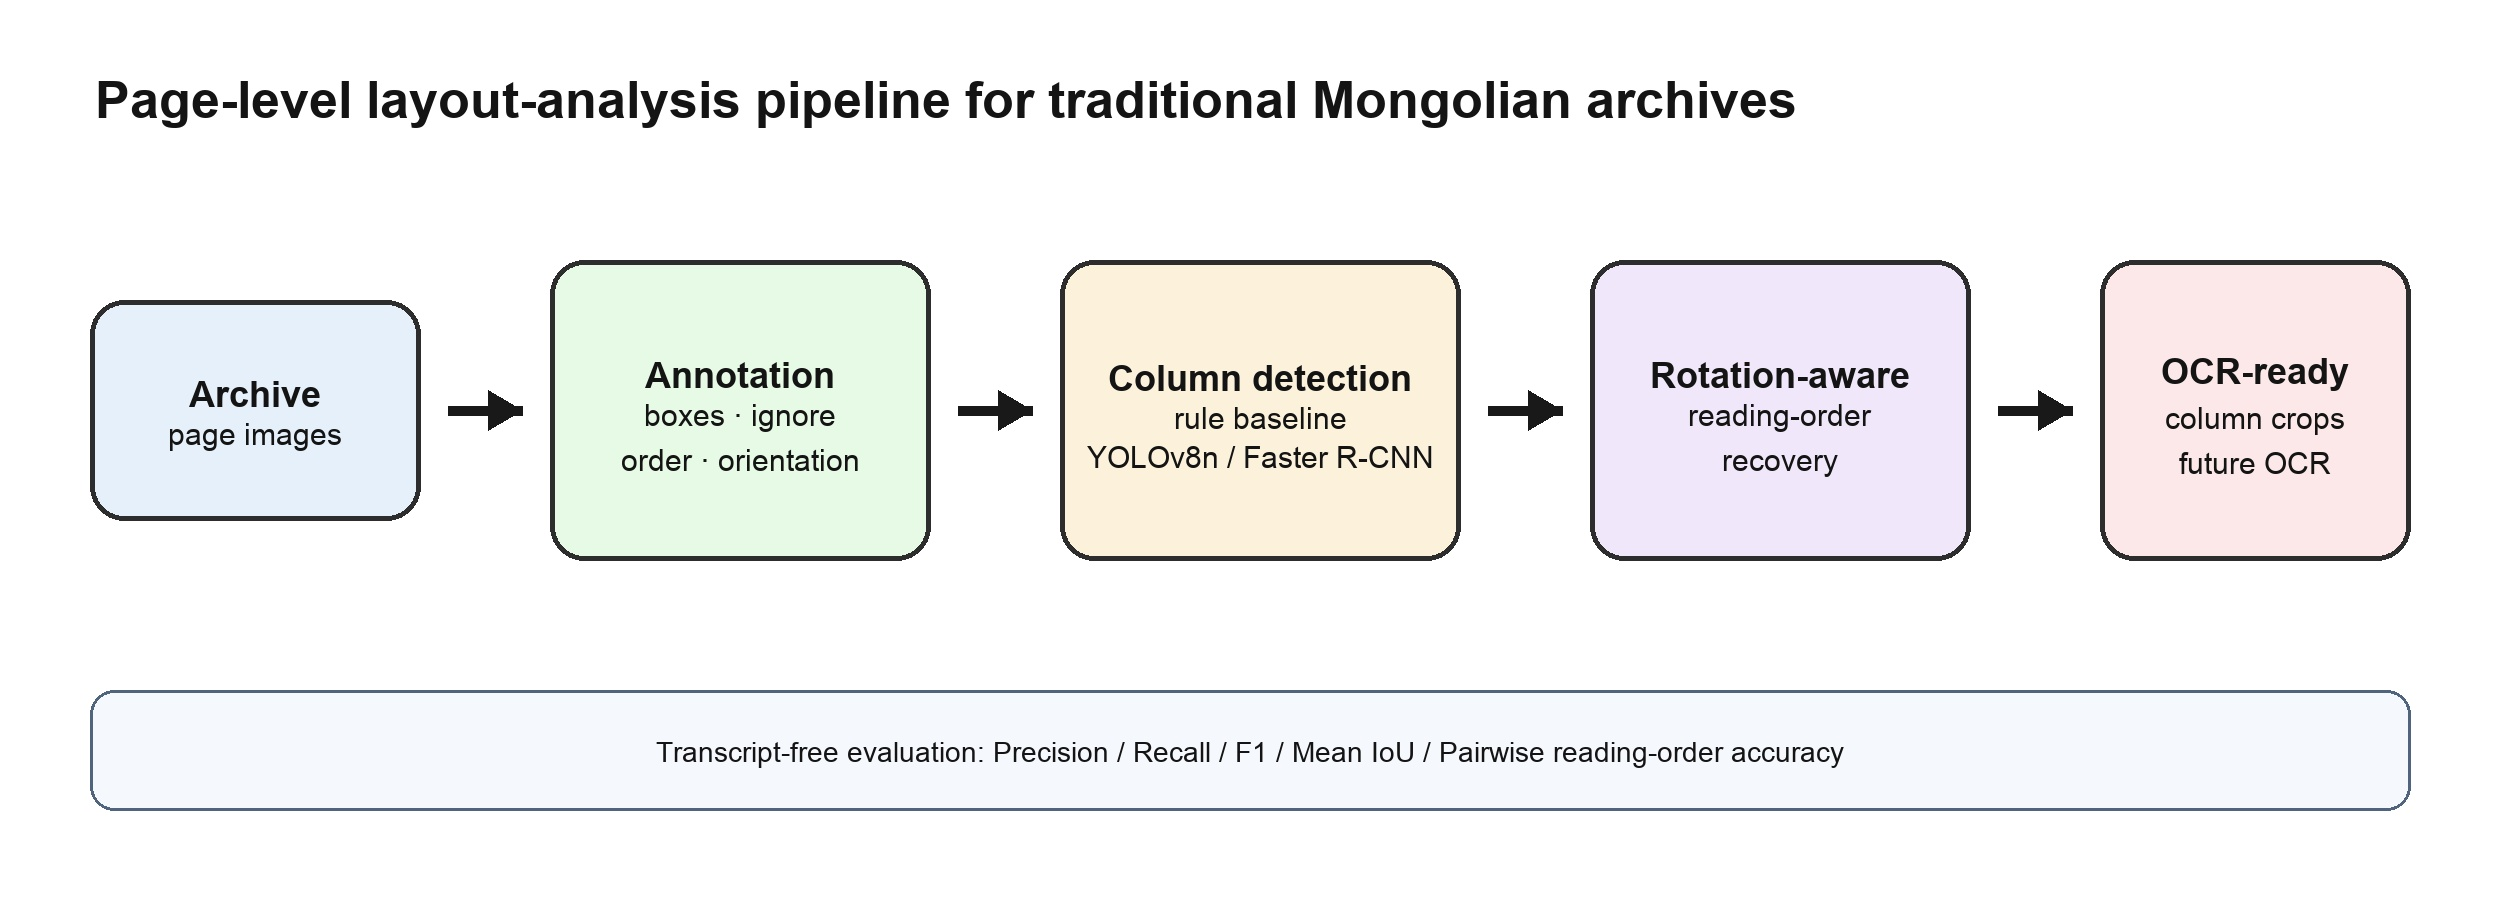
\includegraphics[width=\linewidth]{figures/page_layout_pipeline_overview.jpg}
\caption{Overview of the page-level layout-analysis pipeline. The current study evaluates text-column detection and reading-order recovery without requiring expert text transcription.}
\label{fig:pipeline}
\end{figure}

\section{Related Work}
\textbf{Historical document layout analysis.} Segmentation remains a prerequisite for reliable historical document recognition. Surveys and historical datasets show that degradation, background noise, and handwriting variability make page decomposition difficult~\cite{likforman2007textline,nikolaidou2022survey,gruning2017readbad}. Traditional Mongolian recognition has been studied at word or character level, including online handwriting resources such as MOLHW~\cite{pan2023molhw}, but page-level layout analysis for handwritten historical Mongolian archives remains underexplored.

\textbf{Learning-based document detection.} PubLayNet, DocLayNet, and LayoutParser have promoted reusable learning-based document-layout pipelines~\cite{zhong2019publaynet,pfitzmann2022doclaynet,shen2021layoutparser}. Recent YOLO-style document-layout models also show competitive detection ability in modern document settings~\cite{deng2023yolo,zhao2024doclayout}. These resources mainly target modern printed or PDF-derived pages, whereas our archive pages are handwritten, vertically arranged, and affected by scan rotation and cultural-heritage degradation.

\textbf{Reading-order recovery.} Reading-order recovery is necessary for converting detected regions into structured text. Handwritten document understanding still requires ordering beyond line recognition~\cite{quiros2022reading}, and historical OCR frameworks treat layout analysis, segmentation, and recognition as connected stages~\cite{neudecker2019ocrd}. We therefore evaluate column detection and order recovery independently, and export crops for future recognition once expert transcripts become available.

\section{Dataset and Annotation Protocol}
The dataset contains 62 valid traditional Mongolian archive pages after removing Chinese handwritten archive pages and correcting abnormal scan orientation. The split contains 43 training pages, 8 validation pages, and 11 test pages. The annotations include 904 valid text-column boxes and 122 ignored regions. In internal files the training split was named train\_unlabeled because it has no text transcripts; it nevertheless has layout annotations.

\begin{table}[t]
\centering
\caption{Page-level annotation statistics.}
\label{tab:data_stats}
\begin{tabular}{lrrr}
\toprule
Split & Pages & TextColumn boxes & Ignored boxes \\
\midrule
train & 43 & 637 & 67 \\
val & 8 & 115 & 10 \\
test & 11 & 152 & 45 \\
\midrule
total & 62 & 904 & 122 \\
\bottomrule
\end{tabular}
\end{table}

\begin{table}[t]
\centering
\caption{Dataset distribution statistics over the 62-page corpus. Width, height, and bounding-box dimensions are in pixels.}
\label{tab:dataset_distribution}
\resizebox{\linewidth}{!}{%
\begin{tabular}{lrrrr}
\toprule
Quantity & Min & Max & Mean & Median \\
\midrule
Page width & 4830 & 7396 & 6618.5 & 6794 \\
Page height & 4830 & 9594 & 5698.3 & 4830 \\
Text columns per page & 1 & 27 & 15.0 & 16 \\
Ignore regions per page & 0 & 9 & 2.5 & 2 \\
Column-box width & 109 & 871 & 257.4 & 252 \\
Column-box height & 182 & 8189 & 2873.7 & 3256 \\
\bottomrule
\end{tabular}%
}
\end{table}

Each non-ignored text column is annotated with a bounding box and reading-order index. Ignored regions cover seals, stains, page borders, non-target-language regions, ambiguous fragments, and unseparable artifact--text overlaps. A 5-page independent annotation subset gives text-column box F1@0.5 of 0.852 and mean matched IoU of 0.800; reading-order agreement is lower at 0.677, and Ignore-region agreement is weak, which we treat as a limitation. Pages originally horizontal or upside down are relabeled after rotation so that coordinates match the displayed image.

\begin{figure}[t]
\centering
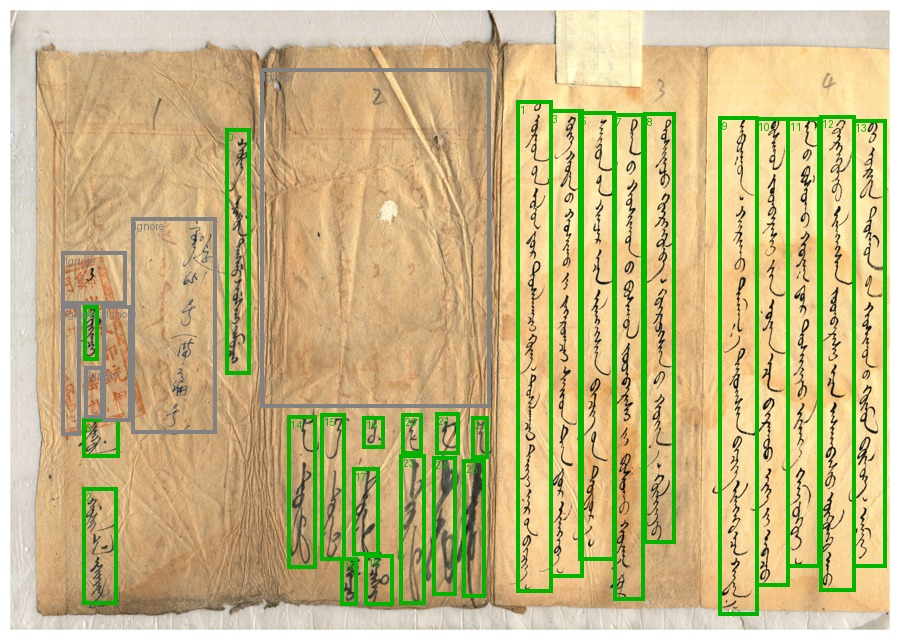
\includegraphics[width=0.78\linewidth]{figures/page_layout_annotation_example.jpg}
\caption{Example of the annotation protocol. Green boxes indicate valid text columns with reading-order indices, while gray boxes indicate ignored regions.}
\label{fig:annotation}
\end{figure}

\section{Method}
\textbf{Rule-based baselines.} We evaluate Sauvola-projection, connected-component grouping, and a stronger heuristic column-extraction baseline. The heuristic baseline applies adaptive binarization, vertical ink-density projection, connected-component filtering, and width, height, and density constraints, followed by overlap merging and left-to-right order assignment. It is interpretable but sensitive to stains, faint ink, and over-merging.

\textbf{Learning-based detectors.} We train YOLOv8n~\cite{jocher2023yolov8} for 50 epochs with image size 960 and batch size 1, initialized from public weights. The confidence threshold 0.35 is selected only on the validation split. We also fine-tune a COCO-pretrained Faster R-CNN MobileNetV3-FPN detector for 5 epochs with max-side 960; threshold 0.80 is selected on validation. Faster R-CNN is not exhaustively optimized, but provides a two-stage detector comparison.

\textbf{Rotation-aware reading order.} For detections $b_i=(x_{1i},y_{1i},x_{2i},y_{2i})$, the column center is $c_i=(x_{1i}+x_{2i})/2$. Detections are sorted by $c_i$ ascending for ordinary pages and descending for pages relabeled after 90-degree rotation. This transparent rule changes only the reading-order field and does not modify detection boxes.

\textbf{Crop-export interface.} The pipeline exports oracle crops from ground-truth boxes and detected crops from learned detections. These crops can be passed to an OCR recognizer after reliable column-level transcripts are added; no CER/WER is reported in the present study.

\section{Experiments}
\subsection{Metrics}
Column detection is evaluated with greedy IoU@0.5 matching. We report precision, recall, F1, mean matched IoU, and pairwise reading-order accuracy over matched columns. Predictions substantially overlapping ignored regions are not counted as false positives. We also report AP@0.50/AP@0.75, complete detection rate, full-page success rate, and page-level bootstrap 95\% confidence intervals. Complete detection requires all valid columns on a page to be matched with no false positives or false negatives; full-page success additionally requires perfect matched-pair reading order.

\subsection{Main Results}
\begin{table}[t]
\centering
\caption{Unified test-set comparison under IoU@0.5 matching. RO Acc. denotes reading-order accuracy.}
\label{tab:main_results}
\resizebox{\linewidth}{!}{%
\begin{tabular}{lccccc}
\toprule
Method & Prec. & Rec. & F1 & Mean IoU & RO Acc. \\
\midrule
Sauvola + projection & 0.344 & 0.276 & 0.307 & 0.644 & 1.000 \\
Connected components & 0.109 & 0.033 & 0.051 & 0.600 & -- \\
Heuristic column extraction & 0.436 & 0.605 & 0.507 & \textbf{0.826} & 0.900 \\
YOLOv8n + rotation-aware order & \textbf{0.956} & 0.717 & 0.820 & 0.770 & \textbf{0.900} \\
Faster R-CNN MobileNet + rotation-aware order & 0.912 & \textbf{0.750} & \textbf{0.823} & 0.738 & 0.818 \\
\bottomrule
\end{tabular}%
}
\end{table}

Table~\ref{tab:main_results} shows that both learned detectors outperform the heuristic baseline. Faster R-CNN obtains the highest IoU@0.5 F1, while YOLOv8n gives the highest reading-order accuracy and precision. The heuristic method has higher mean IoU on matched boxes, but misses many degraded or short columns.

\begin{table}[t]
\centering
\caption{Raw detection counts and approximate confidence-sweep AP on the test split. All methods are evaluated against 152 non-ignored text columns.}
\label{tab:counts_ap}
\resizebox{\linewidth}{!}{%
\begin{tabular}{lrrrrcc}
\toprule
Method & Pred. & TP & FP & FN & AP@0.50 & AP@0.75 \\
\midrule
Heuristic column extraction & 211 & 92 & 119 & 60 & -- & -- \\
YOLOv8n + rotation-aware order & 114 & 109 & 5 & 43 & \textbf{0.921} & \textbf{0.399} \\
Faster R-CNN MobileNet + rotation-aware order & 125 & 114 & 11 & 38 & 0.700 & 0.097 \\
\bottomrule
\end{tabular}%
}
\end{table}

\begin{table}[t]
\centering
\caption{Strict page-level metrics and bootstrap uncertainty on the 11-page test split. Complete detection and full-page success are zero for both evaluated methods.}
\label{tab:strict_ci}
\resizebox{\linewidth}{!}{%
\begin{tabular}{lcccc}
\toprule
Method & Complete det. & Full-page success & F1 95\% CI & Notes \\
\midrule
Heuristic column extraction & 0.000 & 0.000 & [0.427, 0.735] & lower recall \\
YOLOv8n + rotation-aware order & 0.000 & 0.000 & [0.601, 0.866] & higher order accuracy \\
Faster R-CNN MobileNet + rotation-aware order & -- & -- & [0.689, 0.879] & best IoU@0.5 F1 \\
\bottomrule
\end{tabular}%
}
\end{table}

The strict page-level metrics are more demanding than box-level F1. No test page is fully solved: one missed or extra column causes complete detection to fail. Thus, the current system should be interpreted as a candidate crop generator rather than a fully automatic OCR preprocessing solution.

\begin{figure}[t]
\centering
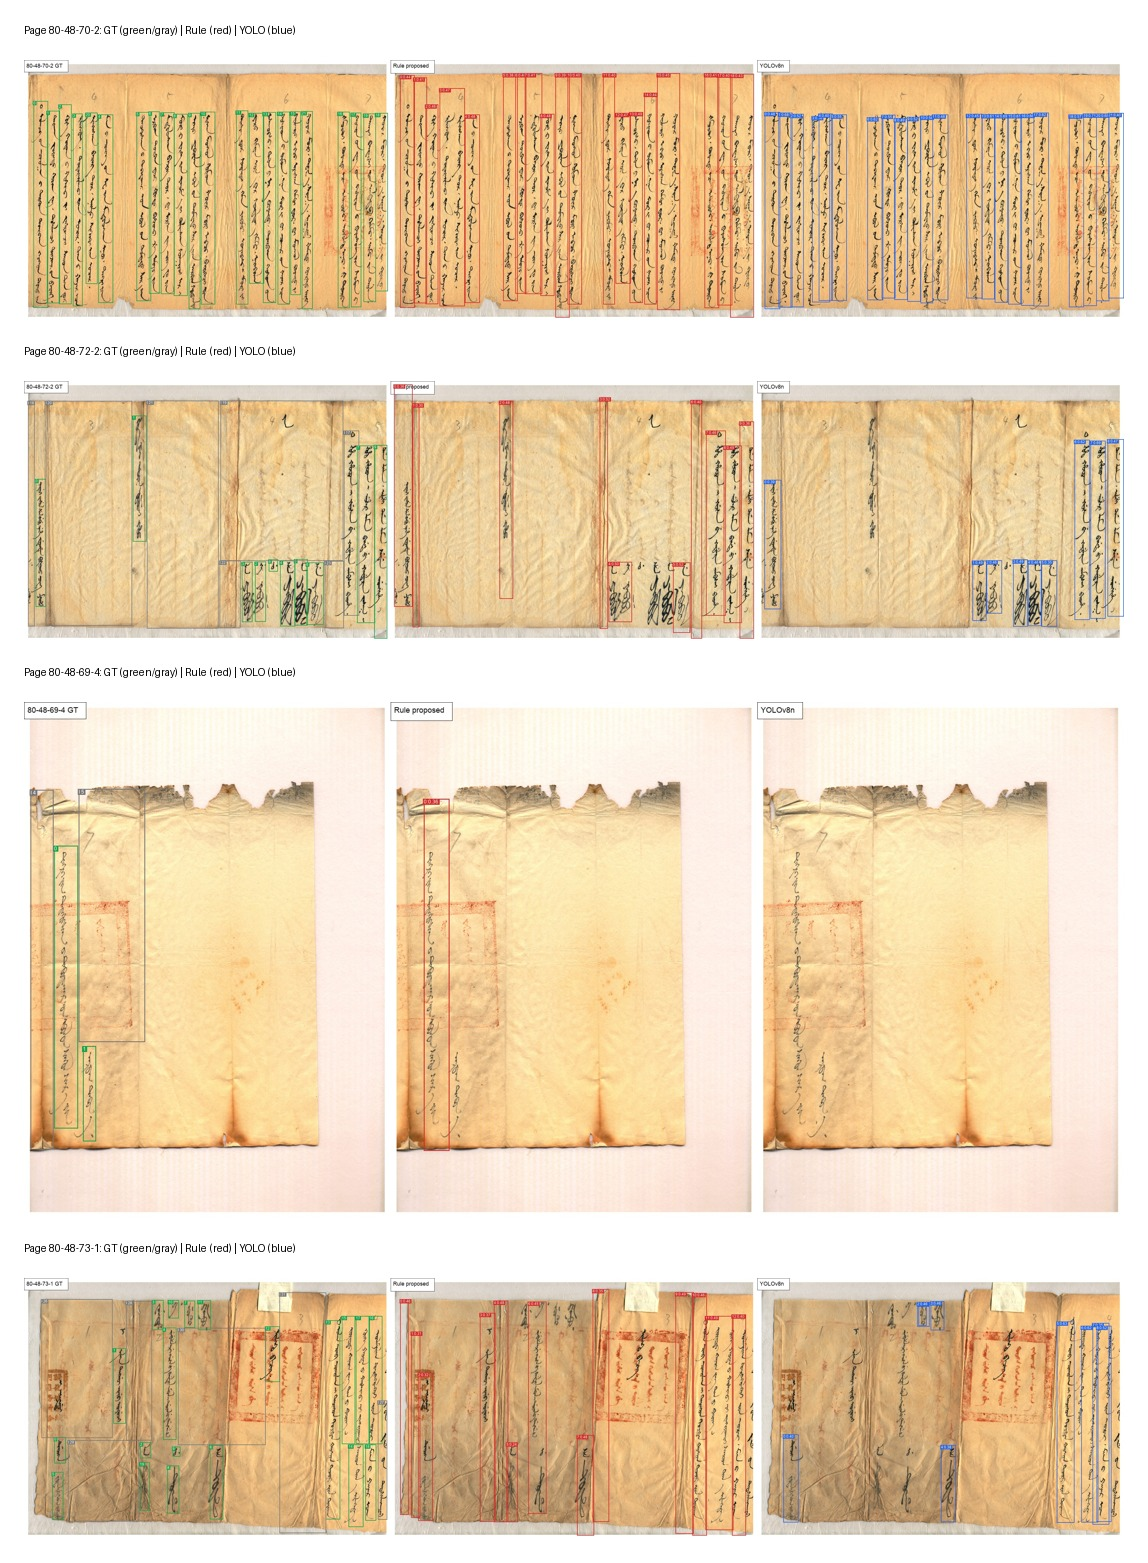
\includegraphics[width=0.88\linewidth]{figures/page_layout_qualitative_failure_montage.jpg}
\caption{Representative comparisons. Each row shows ground truth, rule-based predictions, and YOLOv8n predictions. Green denotes valid text columns, gray ignored regions, red rule-based detections, and blue YOLO detections.}
\label{fig:qualitative}
\end{figure}

\subsection{Ablation and Diagnostics}
On the corrected test labels, ignore-region filtering does not suppress any YOLO predictions, so detection F1 is unchanged in the ablation. Removing rotation-aware ordering leaves detection F1 unchanged; on this small test split, x-sorted order happens to give slightly higher reading-order accuracy than the rotation-aware heuristic. At IoU@0.75, YOLOv8n F1 falls to 0.496 and Faster R-CNN to 0.318, indicating that strict boundary localization remains difficult. Additional diagnostic transfer experiments with RT-DETR and DocLayout-YOLO, together with threshold, inference-size, and column-aware filtering results, are provided in the supplementary material.

\section{Discussion and Limitations}
The main value of the study is a realistic pilot-scale benchmark for a low-resource archival layout problem, not a complete OCR system. The dataset is layout-dense but small, and the 11-page test split yields wide confidence intervals. Several stratified groups contain only one or two pages, so subgroup results should be interpreted only as diagnostic observations. Ignore-region agreement is weak, and the refined subtype guideline needs more examples and annotator training.

The comparison also has methodological limits. YOLOv8n and Faster R-CNN are trained with different budgets, and Faster R-CNN is not exhaustively optimized; its strong IoU@0.5 result suggests that two-stage detection deserves future compute-matched investigation. The AP@0.75 and full-page-success results show that boundary precision and complete page handling remain unresolved. Future work will add a small expert-transcribed subset to enable oracle-crop and detected-crop OCR case studies.

\section{Conclusion}
We presented a pilot-scale page-level layout-analysis benchmark for traditional Mongolian historical archives under a realistic condition where expert text transcription is unavailable. Learning-based detectors with rotation-aware ordering outperform heuristic extraction on the independent test split. YOLOv8n reaches 0.820 F1 and 0.900 reading-order accuracy, while Faster R-CNN reaches 0.823 F1. However, complete detection and full-page success remain 0 on the current test split. The present system should therefore be viewed as a crop-export-ready candidate generator and an evaluation protocol for future traditional Mongolian archival OCR, not as a fully automatic end-to-end OCR solution.

\section*{Data Availability}
The project materials include the annotation schema, page-level annotation files, split manifests, evaluation scripts, trained-detector configuration notes, and generated prediction files. These non-image research artifacts can be shared with reviewers or released publicly when allowed by project policy. The archive images are subject to institutional access constraints; complete reproduction therefore requires authorized access to the original archive images.

\section*{Author Contributions}
Lanying Liang: Conceptualization, Data Curation, Writing -- Original Draft. Yuefeng Liu: Methodology, Software, Validation, Writing -- Review \& Editing, Supervision.

\section*{Ethics Statement}
This study uses historical archive images for document analysis and digital preservation. No personal intervention or modern human-subject experiment is involved. The work does not attempt to infer sensitive attributes of living individuals.

\section*{Funding}
This work was supported by the National Natural Science Foundation of China (Grant No. 62341604), the Science and Technology Project of Inner Mongolia Autonomous Region Archives Bureau (Grant No. 2022-36), the China Scholarship Council (Grant No. 202408150080), and the General Project of the 14th Five-Year Plan for Educational Science of Inner Mongolia Autonomous Region (Grant No. NGJGH2025013).

\begin{thebibliography}{10}

\bibitem{likforman2007textline}
L. Likforman-Sulem, A. Zahour, and B. Taconet, ``Text line segmentation of historical documents: a survey,'' \emph{International Journal on Document Analysis and Recognition}, vol. 9, pp. 123--138, 2007. doi: 10.1007/s10032-006-0023-z.

\bibitem{nikolaidou2022survey}
K. Nikolaidou, M. Seuret, H. Mokayed, and M. Liwicki, ``A survey of historical document image datasets,'' \emph{International Journal on Document Analysis and Recognition}, vol. 25, pp. 305--338, 2022. doi: 10.1007/s10032-022-00405-8.

\bibitem{gruning2017readbad}
T. Gr\"uning, R. Labahn, M. Diem, F. Kleber, and S. Fiel, ``READ-BAD: A new dataset and evaluation scheme for baseline detection in archival documents,'' arXiv:1705.03311, 2017.

\bibitem{zhong2019publaynet}
X. Zhong, J. Tang, and A. J. Yepes, ``PubLayNet: largest dataset ever for document layout analysis,'' in \emph{Proc. International Conference on Document Analysis and Recognition}, 2019, pp. 1015--1022. doi: 10.1109/ICDAR.2019.00166.

\bibitem{pfitzmann2022doclaynet}
B. Pfitzmann, C. Auer, M. Dolfi, A. S. Nassar, and P. W. J. Staar, ``DocLayNet: A large human-annotated dataset for document-layout analysis,'' in \emph{Proc. ACM SIGKDD International Conference on Knowledge Discovery and Data Mining}, 2022. doi: 10.1145/3534678.3539043.

\bibitem{shen2021layoutparser}
Z. Shen, R. Zhang, M. Dell, B. C. G. Lee, J. Carlson, and W. Li, ``LayoutParser: A unified toolkit for deep learning based document image analysis,'' in \emph{Document Analysis and Recognition -- ICDAR 2021}, LNCS 12821, pp. 131--146, 2021. doi: 10.1007/978-3-030-86549-8\_9.

\bibitem{quiros2022reading}
L. Quir\'os and E. Vidal, ``Reading order detection on handwritten documents,'' \emph{Neural Computing and Applications}, vol. 34, pp. 9593--9611, 2022. doi: 10.1007/s00521-022-06948-5.

\bibitem{neudecker2019ocrd}
C. Neudecker, K. Baierer, M. Federbusch, M. Boenig, K.-M. W\"urzner, V. Hartmann, and E. Herrmann, ``OCR-D: An end-to-end open source OCR framework for historical printed documents,'' in \emph{Proc. DATeCH2019}, 2019, pp. 53--58. doi: 10.1145/3322905.3322917.


\bibitem{pan2023molhw}
Y. Pan, D. Fan, H. Wu, and D. Teng, ``A new dataset for Mongolian online handwritten recognition,'' \emph{Scientific Reports}, vol. 13, article 26, 2023. doi: 10.1038/s41598-022-27267-8.

\bibitem{deng2023yolo}
Q. Deng, M. Ibrayim, A. Hamdulla, and C. Zhang, ``The YOLO model that still excels in document layout analysis,'' \emph{Signal, Image and Video Processing}, vol. 18, no. 2, pp. 1539--1548, 2024. doi: 10.1007/s11760-023-02838-y.

\bibitem{zhao2024doclayout}
Z. Zhao, H. Kang, B. Wang, and C. He, ``DocLayout-YOLO: Enhancing document layout analysis through diverse synthetic data and global-to-local adaptive perception,'' arXiv:2410.12628, 2024.

\bibitem{jocher2023yolov8}
G. Jocher, A. Chaurasia, and J. Qiu, ``Ultralytics YOLOv8,'' software, version 8.0.0, 2023. Available: \url{https://github.com/ultralytics/ultralytics}.

\end{thebibliography}


\end{document}
